Cette section présente les figures principales du document
et comment les utiliser. Il est important de savoir que
les figures sont des éléments flottants. Cela signifie 
qu'elles peuvent être placées à un endroit différent
de celui où elles sont déclarées dans le code, c'est un 
point important à garder en tête.

\subsection{Les figures}\label{subsec:latex_figures}
Les figures sont des éléments flottants qui peuvent être placés
par rapport à une position donnée dans le document. Il est possible
de les placer à des endroits différents en utilisant des options de placement
comme \texttt{h} (ici), \texttt{t} (en haut de la page), \texttt{b} (en bas de la page).

Le code suivant insère la figure~\ref{fig:example_figure} qui le suit:

\inputminted[frame=single,framesep=4pt,breaklines,linenos]{latex}{./5_Figures/figure1_code.tex}

\begin{figure}[!htb]
    \centering
    \fbox{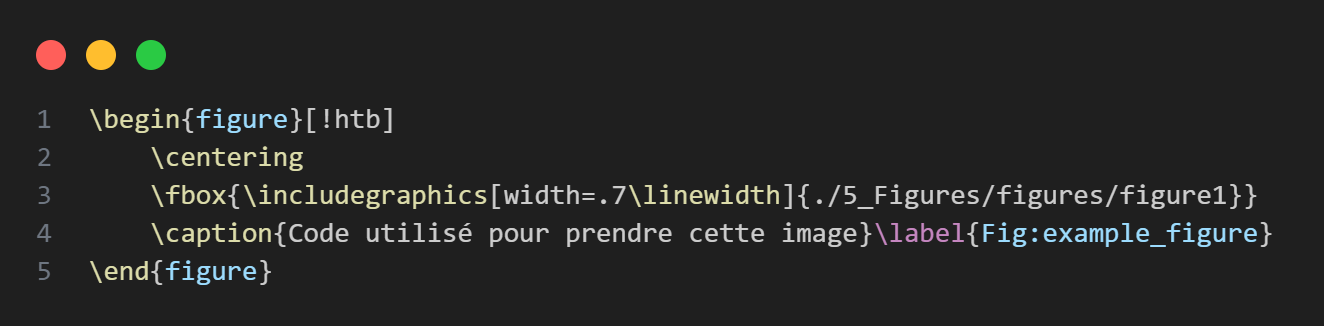
\includegraphics[width=.7\linewidth]{./5_Figures/figures/figure1}}
    \caption{Code utilisé pour prendre cette image}\label{fig:example_figure}
\end{figure}